% Created by tikzDevice version 0.12.6 on 2026-05-14 21:28:22
% !TEX encoding = UTF-8 Unicode
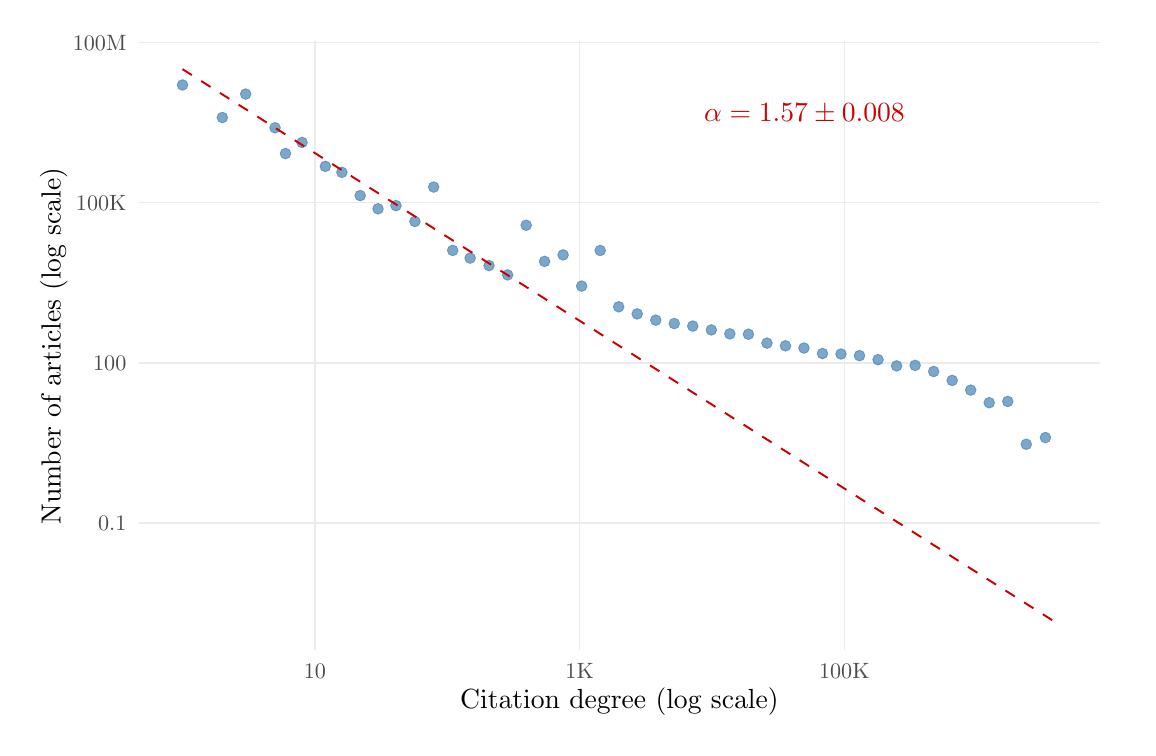
\begin{tikzpicture}[x=1pt,y=1pt]
\definecolor{fillColor}{RGB}{255,255,255}
\path[use as bounding box,fill=fillColor,fill opacity=0.00] (0,0) rectangle (397.48,252.94);
\begin{scope}
\path[clip] (  0.00,  0.00) rectangle (397.48,252.94);
\definecolor{fillColor}{RGB}{255,255,255}

\path[fill=fillColor] (  0.00,  0.00) rectangle (397.48,252.94);
\end{scope}
\begin{scope}
\path[clip] ( 40.16, 27.90) rectangle (387.48,247.95);
\definecolor{drawColor}{gray}{0.92}

\path[draw=drawColor,line width= 0.5pt,line join=round] ( 40.16, 73.90) --
	(387.48, 73.90);

\path[draw=drawColor,line width= 0.5pt,line join=round] ( 40.16,131.80) --
	(387.48,131.80);

\path[draw=drawColor,line width= 0.5pt,line join=round] ( 40.16,189.69) --
	(387.48,189.69);

\path[draw=drawColor,line width= 0.5pt,line join=round] ( 40.16,247.59) --
	(387.48,247.59);

\path[draw=drawColor,line width= 0.5pt,line join=round] (103.77, 27.90) --
	(103.77,247.95);

\path[draw=drawColor,line width= 0.5pt,line join=round] (199.43, 27.90) --
	(199.43,247.95);

\path[draw=drawColor,line width= 0.5pt,line join=round] (295.08, 27.90) --
	(295.08,247.95);
\definecolor{drawColor}{RGB}{70,130,180}
\definecolor{fillColor}{RGB}{70,130,180}

\path[draw=drawColor,draw opacity=0.70,line width= 0.3pt,line join=round,line cap=round,fill=fillColor,fill opacity=0.70] ( 55.95,232.23) circle (  1.93);

\path[draw=drawColor,draw opacity=0.70,line width= 0.3pt,line join=round,line cap=round,fill=fillColor,fill opacity=0.70] ( 70.34,220.47) circle (  1.93);

\path[draw=drawColor,draw opacity=0.70,line width= 0.3pt,line join=round,line cap=round,fill=fillColor,fill opacity=0.70] ( 78.77,228.95) circle (  1.93);

\path[draw=drawColor,draw opacity=0.70,line width= 0.3pt,line join=round,line cap=round,fill=fillColor,fill opacity=0.70] ( 89.38,216.77) circle (  1.93);

\path[draw=drawColor,draw opacity=0.70,line width= 0.3pt,line join=round,line cap=round,fill=fillColor,fill opacity=0.70] ( 93.16,207.44) circle (  1.93);

\path[draw=drawColor,draw opacity=0.70,line width= 0.3pt,line join=round,line cap=round,fill=fillColor,fill opacity=0.70] ( 99.14,211.46) circle (  1.93);

\path[draw=drawColor,draw opacity=0.70,line width= 0.3pt,line join=round,line cap=round,fill=fillColor,fill opacity=0.70] (107.56,202.83) circle (  1.93);

\path[draw=drawColor,draw opacity=0.70,line width= 0.3pt,line join=round,line cap=round,fill=fillColor,fill opacity=0.70] (113.54,200.67) circle (  1.93);

\path[draw=drawColor,draw opacity=0.70,line width= 0.3pt,line join=round,line cap=round,fill=fillColor,fill opacity=0.70] (120.15,192.27) circle (  1.93);

\path[draw=drawColor,draw opacity=0.70,line width= 0.3pt,line join=round,line cap=round,fill=fillColor,fill opacity=0.70] (126.59,187.49) circle (  1.93);

\path[draw=drawColor,draw opacity=0.70,line width= 0.3pt,line join=round,line cap=round,fill=fillColor,fill opacity=0.70] (133.08,188.63) circle (  1.93);

\path[draw=drawColor,draw opacity=0.70,line width= 0.3pt,line join=round,line cap=round,fill=fillColor,fill opacity=0.70] (139.92,182.92) circle (  1.93);

\path[draw=drawColor,draw opacity=0.70,line width= 0.3pt,line join=round,line cap=round,fill=fillColor,fill opacity=0.70] (146.70,195.35) circle (  1.93);

\path[draw=drawColor,draw opacity=0.70,line width= 0.3pt,line join=round,line cap=round,fill=fillColor,fill opacity=0.70] (153.58,172.45) circle (  1.93);

\path[draw=drawColor,draw opacity=0.70,line width= 0.3pt,line join=round,line cap=round,fill=fillColor,fill opacity=0.70] (159.88,169.68) circle (  1.93);

\path[draw=drawColor,draw opacity=0.70,line width= 0.3pt,line join=round,line cap=round,fill=fillColor,fill opacity=0.70] (166.71,166.98) circle (  1.93);

\path[draw=drawColor,draw opacity=0.70,line width= 0.3pt,line join=round,line cap=round,fill=fillColor,fill opacity=0.70] (173.43,163.60) circle (  1.93);

\path[draw=drawColor,draw opacity=0.70,line width= 0.3pt,line join=round,line cap=round,fill=fillColor,fill opacity=0.70] (180.13,181.55) circle (  1.93);

\path[draw=drawColor,draw opacity=0.70,line width= 0.3pt,line join=round,line cap=round,fill=fillColor,fill opacity=0.70] (186.78,168.48) circle (  1.93);

\path[draw=drawColor,draw opacity=0.70,line width= 0.3pt,line join=round,line cap=round,fill=fillColor,fill opacity=0.70] (193.48,170.83) circle (  1.93);

\path[draw=drawColor,draw opacity=0.70,line width= 0.3pt,line join=round,line cap=round,fill=fillColor,fill opacity=0.70] (200.18,159.56) circle (  1.93);

\path[draw=drawColor,draw opacity=0.70,line width= 0.3pt,line join=round,line cap=round,fill=fillColor,fill opacity=0.70] (206.87,172.43) circle (  1.93);

\path[draw=drawColor,draw opacity=0.70,line width= 0.3pt,line join=round,line cap=round,fill=fillColor,fill opacity=0.70] (213.56,152.07) circle (  1.93);

\path[draw=drawColor,draw opacity=0.70,line width= 0.3pt,line join=round,line cap=round,fill=fillColor,fill opacity=0.70] (220.25,149.51) circle (  1.93);

\path[draw=drawColor,draw opacity=0.70,line width= 0.3pt,line join=round,line cap=round,fill=fillColor,fill opacity=0.70] (226.96,147.25) circle (  1.93);

\path[draw=drawColor,draw opacity=0.70,line width= 0.3pt,line join=round,line cap=round,fill=fillColor,fill opacity=0.70] (233.64,146.02) circle (  1.93);

\path[draw=drawColor,draw opacity=0.70,line width= 0.3pt,line join=round,line cap=round,fill=fillColor,fill opacity=0.70] (240.33,145.12) circle (  1.93);

\path[draw=drawColor,draw opacity=0.70,line width= 0.3pt,line join=round,line cap=round,fill=fillColor,fill opacity=0.70] (247.03,143.72) circle (  1.93);

\path[draw=drawColor,draw opacity=0.70,line width= 0.3pt,line join=round,line cap=round,fill=fillColor,fill opacity=0.70] (253.72,142.30) circle (  1.93);

\path[draw=drawColor,draw opacity=0.70,line width= 0.3pt,line join=round,line cap=round,fill=fillColor,fill opacity=0.70] (260.44,142.17) circle (  1.93);

\path[draw=drawColor,draw opacity=0.70,line width= 0.3pt,line join=round,line cap=round,fill=fillColor,fill opacity=0.70] (267.14,138.96) circle (  1.93);

\path[draw=drawColor,draw opacity=0.70,line width= 0.3pt,line join=round,line cap=round,fill=fillColor,fill opacity=0.70] (273.82,137.97) circle (  1.93);

\path[draw=drawColor,draw opacity=0.70,line width= 0.3pt,line join=round,line cap=round,fill=fillColor,fill opacity=0.70] (280.51,137.18) circle (  1.93);

\path[draw=drawColor,draw opacity=0.70,line width= 0.3pt,line join=round,line cap=round,fill=fillColor,fill opacity=0.70] (287.20,135.19) circle (  1.93);

\path[draw=drawColor,draw opacity=0.70,line width= 0.3pt,line join=round,line cap=round,fill=fillColor,fill opacity=0.70] (293.89,135.02) circle (  1.93);

\path[draw=drawColor,draw opacity=0.70,line width= 0.3pt,line join=round,line cap=round,fill=fillColor,fill opacity=0.70] (300.58,134.43) circle (  1.93);

\path[draw=drawColor,draw opacity=0.70,line width= 0.3pt,line join=round,line cap=round,fill=fillColor,fill opacity=0.70] (307.28,132.97) circle (  1.93);

\path[draw=drawColor,draw opacity=0.70,line width= 0.3pt,line join=round,line cap=round,fill=fillColor,fill opacity=0.70] (313.99,130.72) circle (  1.93);

\path[draw=drawColor,draw opacity=0.70,line width= 0.3pt,line join=round,line cap=round,fill=fillColor,fill opacity=0.70] (320.68,130.91) circle (  1.93);

\path[draw=drawColor,draw opacity=0.70,line width= 0.3pt,line join=round,line cap=round,fill=fillColor,fill opacity=0.70] (327.38,128.69) circle (  1.93);

\path[draw=drawColor,draw opacity=0.70,line width= 0.3pt,line join=round,line cap=round,fill=fillColor,fill opacity=0.70] (334.06,125.47) circle (  1.93);

\path[draw=drawColor,draw opacity=0.70,line width= 0.3pt,line join=round,line cap=round,fill=fillColor,fill opacity=0.70] (340.76,121.98) circle (  1.93);

\path[draw=drawColor,draw opacity=0.70,line width= 0.3pt,line join=round,line cap=round,fill=fillColor,fill opacity=0.70] (347.45,117.42) circle (  1.93);

\path[draw=drawColor,draw opacity=0.70,line width= 0.3pt,line join=round,line cap=round,fill=fillColor,fill opacity=0.70] (354.15,117.88) circle (  1.93);

\path[draw=drawColor,draw opacity=0.70,line width= 0.3pt,line join=round,line cap=round,fill=fillColor,fill opacity=0.70] (360.84,102.40) circle (  1.93);

\path[draw=drawColor,draw opacity=0.70,line width= 0.3pt,line join=round,line cap=round,fill=fillColor,fill opacity=0.70] (367.76,104.82) circle (  1.93);
\definecolor{drawColor}{RGB}{205,0,0}

\path[draw=drawColor,line width= 0.7pt,dash pattern=on 4pt off 4pt ,line join=round] ( 55.95,237.94) --
	( 59.14,235.92) --
	( 62.33,233.90) --
	( 65.52,231.88) --
	( 68.70,229.86) --
	( 71.89,227.84) --
	( 75.08,225.82) --
	( 78.27,223.80) --
	( 81.46,221.78) --
	( 84.65,219.76) --
	( 87.84,217.74) --
	( 91.03,215.72) --
	( 94.22,213.69) --
	( 97.41,211.67) --
	(100.60,209.65) --
	(103.79,207.63) --
	(106.98,205.61) --
	(110.17,203.59) --
	(113.36,201.57) --
	(116.55,199.55) --
	(119.74,197.53) --
	(122.92,195.51) --
	(126.11,193.49) --
	(129.30,191.47) --
	(132.49,189.45) --
	(135.68,187.43) --
	(138.87,185.41) --
	(142.06,183.39) --
	(145.25,181.36) --
	(148.44,179.34) --
	(151.63,177.32) --
	(154.82,175.30) --
	(158.01,173.28) --
	(161.20,171.26) --
	(164.39,169.24) --
	(167.58,167.22) --
	(170.77,165.20) --
	(173.95,163.18) --
	(177.14,161.16) --
	(180.33,159.14) --
	(183.52,157.12) --
	(186.71,155.10) --
	(189.90,153.08) --
	(193.09,151.05) --
	(196.28,149.03) --
	(199.47,147.01) --
	(202.66,144.99) --
	(205.85,142.97) --
	(209.04,140.95) --
	(212.23,138.93) --
	(215.42,136.91) --
	(218.61,134.89) --
	(221.80,132.87) --
	(224.99,130.85) --
	(228.17,128.83) --
	(231.36,126.81) --
	(234.55,124.79) --
	(237.74,122.77) --
	(240.93,120.75) --
	(244.12,118.72) --
	(247.31,116.70) --
	(250.50,114.68) --
	(253.69,112.66) --
	(256.88,110.64) --
	(260.07,108.62) --
	(263.26,106.60) --
	(266.45,104.58) --
	(269.64,102.56) --
	(272.83,100.54) --
	(276.02, 98.52) --
	(279.21, 96.50) --
	(282.39, 94.48) --
	(285.58, 92.46) --
	(288.77, 90.44) --
	(291.96, 88.41) --
	(295.15, 86.39) --
	(298.34, 84.37) --
	(301.53, 82.35) --
	(304.72, 80.33) --
	(307.91, 78.31) --
	(311.10, 76.29) --
	(314.29, 74.27) --
	(317.48, 72.25) --
	(320.67, 70.23) --
	(323.86, 68.21) --
	(327.05, 66.19) --
	(330.24, 64.17) --
	(333.42, 62.15) --
	(336.61, 60.13) --
	(339.80, 58.10) --
	(342.99, 56.08) --
	(346.18, 54.06) --
	(349.37, 52.04) --
	(352.56, 50.02) --
	(355.75, 48.00) --
	(358.94, 45.98) --
	(362.13, 43.96) --
	(365.32, 41.94) --
	(368.51, 39.92) --
	(371.70, 37.90);

\node[text=drawColor,anchor=base,inner sep=0pt, outer sep=0pt, scale=  1.00] at (280.68,219.05) {$\alpha = 1.57 \pm 0.008$};
\end{scope}
\begin{scope}
\path[clip] (  0.00,  0.00) rectangle (397.48,252.94);
\definecolor{drawColor}{gray}{0.30}

\node[text=drawColor,anchor=base east,inner sep=0pt, outer sep=0pt, scale=  0.80] at ( 35.66, 71.14) {0.1};

\node[text=drawColor,anchor=base east,inner sep=0pt, outer sep=0pt, scale=  0.80] at ( 35.66,129.04) {100};

\node[text=drawColor,anchor=base east,inner sep=0pt, outer sep=0pt, scale=  0.80] at ( 35.66,186.94) {100K};

\node[text=drawColor,anchor=base east,inner sep=0pt, outer sep=0pt, scale=  0.80] at ( 35.66,244.84) {100M};
\end{scope}
\begin{scope}
\path[clip] (  0.00,  0.00) rectangle (397.48,252.94);
\definecolor{drawColor}{gray}{0.30}

\node[text=drawColor,anchor=base,inner sep=0pt, outer sep=0pt, scale=  0.80] at (103.77, 17.89) {10};

\node[text=drawColor,anchor=base,inner sep=0pt, outer sep=0pt, scale=  0.80] at (199.43, 17.89) {1K};

\node[text=drawColor,anchor=base,inner sep=0pt, outer sep=0pt, scale=  0.80] at (295.08, 17.89) {100K};
\end{scope}
\begin{scope}
\path[clip] (  0.00,  0.00) rectangle (397.48,252.94);
\definecolor{drawColor}{RGB}{0,0,0}

\node[text=drawColor,anchor=base,inner sep=0pt, outer sep=0pt, scale=  1.00] at (213.82,  6.94) {Citation degree (log scale)};
\end{scope}
\begin{scope}
\path[clip] (  0.00,  0.00) rectangle (397.48,252.94);
\definecolor{drawColor}{RGB}{0,0,0}

\node[text=drawColor,rotate= 90.00,anchor=base,inner sep=0pt, outer sep=0pt, scale=  1.00] at ( 11.89,137.92) {Number of articles (log scale)};
\end{scope}
\end{tikzpicture}
